\documentclass{scrbook}

%!TEX root = thesis.tex

% Set german to default language and load english as well
\usepackage[english,ngerman]{babel}

% Set UTF8 as input encoding
\usepackage[utf8]{inputenc}

% Set T1 as font encoding
\usepackage[T1]{fontenc}
% Load a slightly more modern font
\usepackage{lmodern}
% Use the symbol collection textcomp, which is needed by listings.
\usepackage{textcomp}
% Load a better font for monospace.
\usepackage{courier}
% Load package to configure header and footer
\usepackage{scrlayer-scrpage}

% Set some options regarding the document layout. See KOMA guide
\KOMAoptions{%
  paper=a4,
  fontsize=12pt,
  parskip=half,
  headings=big,
  BCOR=1cm,
  headsepline,
  %headsepline=0.5pt,
  chapterprefix=true,
  numbers=noendperiod,
  DIV=12}

% do not align bottom of pages
\raggedbottom

% show page layout with \layout
\usepackage{layout}

% set table caption to be on top of tables
\usepackage{floatrow}
\floatsetup[table]{capposition=top}

% set style of captions
\setcapindent{0pt} % do not indent second line of captions
\setkomafont{caption}{\small}
\setkomafont{captionlabel}{\bfseries}
\setcapwidth[c]{0.9\textwidth}

% set the style of the bibliography
\bibliographystyle{unsrt}

% load extended tabulars used in the list of abbreviation
\usepackage{tabularx}

% load the color package and enable colored tables
\usepackage[table]{xcolor}
\usepackage{booktabs}

% define new environment for zebra tables
\newcommand{\mainrowcolors}{\rowcolors{1}{maincolor!25}{maincolor!5}}
\newenvironment{zebratabular}{\mainrowcolors\begin{tabular}}{\end{tabular}}
\newcommand{\setrownumber}[1]{\global\rownum#1\relax}
\newcommand{\headerrow}{\rowcolor{maincolor!20}\setrownumber1}

% add main color to section headers
\addtokomafont{chapter}{\color{maincolor}}
\addtokomafont{section}{\color{maincolor}}
\addtokomafont{subsection}{\color{maincolor}}
\addtokomafont{subsubsection}{\color{maincolor}}
\addtokomafont{paragraph}{\color{maincolor}}

% do not print numbers next to each formula
\usepackage{mathtools}
%\mathtoolsset{showonlyrefs}

% left align formulas
%\makeatletter
%\@fleqntrue\let\mathindent\@mathmargin \@mathmargin=\leftmargini
%\makeatother

% Allow page breaks in align environments
\allowdisplaybreaks

% header and footer
\pagestyle{scrheadings}
\setkomafont{pagenumber}{\normalfont\sffamily\color{maincolor}}
\setkomafont{pageheadfoot}{\normalfont\sffamily}
\setkomafont{headsepline}{\color{maincolor}}

% set text height
\setlength{\textheight}{1.05\textheight}

% German guillemets quotes
\usepackage[german=guillemets]{csquotes}

% load TikZ to draw diagrams
\usepackage{tikz}

% load additional libraries for TikZ
\usetikzlibrary{%
  automata,%
  positioning,%
}

% set some default options for TikZ -- in this case for automata
\tikzset{
  every state/.style={
    draw=maincolor,
    thick,
    fill=maincolor!18,
    minimum size=0pt
  }
}

% load listings package to typeset sourcecode
\usepackage{listings}

% set some options for the listings package
\lstset{%
  upquote=true,%
  showstringspaces=false,%
  captionpos=b,%
  basicstyle=\ttfamily,%
  keywordstyle=\color{keywordcolor}\slshape,%
  commentstyle=\color{commentcolor}\itshape,%
  stringstyle=\color{stringcolor}}
\renewcommand{\lstlistingname}{Quelltext}
\renewcommand{\lstlistlistingname}{Quelltextverzeichnis}

% enable german umlauts in listings
\lstset{
  literate={ö}{{\"o}}1
           {Ö}{{\"O}}1
           {ä}{{\"a}}1
           {Ä}{{\"A}}1
           {ü}{{\"u}}1
           {Ü}{{\"U}}1
           {ß}{{\ss}}1
}

% define style for pseudo code
\lstdefinestyle{pseudo}{language={},%
  basicstyle=\normalfont,%
  morecomment=[l]{//},%
  morekeywords={for,to,while,do,if,then,else},%
  mathescape=true,%
  columns=fullflexible}

% load the AMS math library to typeset formulas
\usepackage{amsmath}
\usepackage{amsthm}
\usepackage{thmtools}
\usepackage{amssymb}

% load SI unit package for beautiful units
\usepackage{siunitx}

% load the paralist library to use compactitem and compactenum environment
\usepackage{paralist}

% load varioref and hyperref to create nicer references using vref
\usepackage[ngerman]{varioref}
\PassOptionsToPackage{hyphens}{url} % allow line break at hyphens in URLs
\usepackage{hyperref}

% setup hyperref
\hypersetup{breaklinks=true,
            pdfborder={0 0 0},
            ngerman,
            pdfhighlight={/N},
            pdfdisplaydoctitle=true}

% Fix bugs in some package, e.g. listings and hyperref
\usepackage{scrhack}

% Allow todos
\usepackage{todonotes}

% define german names for referenced elements
% (vref automatically inserts these names in front of the references)
\labelformat{figure}{Abbildung\ #1}
\labelformat{table}{Tabelle\ #1}
\labelformat{appendix}{Anhang\ #1}
\labelformat{chapter}{Kapitel\ #1}
\labelformat{section}{Abschnitt\ #1}
\labelformat{subsection}{Unterabschnitt\ #1}
\labelformat{subsubsection}{Unterunterabschnitt\ #1}
\AtBeginDocument{\labelformat{lstlisting}{Quelltext\ #1}}

% define theorem environments
\declaretheorem[numberwithin=chapter,style=plain]{Theorem}
\labelformat{Theorem}{Theorem\ #1}

\declaretheorem[sibling=Theorem,style=plain]{Lemma}
\labelformat{Lemma}{Lemma\ #1}

\declaretheorem[sibling=Theorem,style=plain]{Korollar}
\labelformat{Korollar}{Korollar\ #1}

\declaretheorem[sibling=Theorem,style=definition]{Definition}
\labelformat{Definition}{Definition\ #1}

\declaretheorem[sibling=Theorem,style=definition]{Beispiel}
\labelformat{Beispiel}{Beispiel\ #1}

\declaretheorem[sibling=Theorem,style=definition]{Bemerkung}
\labelformat{Bemerkung}{Bemerkung\ #1}

\input{macros}

% Set title and author used in the PDF meta data
\hypersetup{
  pdftitle={Wie schreibe ich eine Masterarbeit?},
  pdfauthor={Erika Mustermann}
}

% Depending on which of the following two color schemes you import your thesis will be in color or grayscale. I recommend to generate a colored version as a PDF and a grayscale version for printing.

%\input{schema-color}
\input{schema-gray}

% Abgabedatum
\newcommand{\duedate}{15. Juli 2016}

\begin{document}
  \frontmatter
  %!TEX root = thesis.tex

\begin{titlepage}
  \thispagestyle{empty}

  %\vskip1cm

 %\pgfimage[height=2.5cm]{uni-logo-example\imagesuffix}
 \pgfimage[height=2.5cm]{images/template/Institutslogo.png}

  \vspace{0.2cm}
{\large\emph{Direktor:} Prof. Dr. C. Hübner}\vspace{0.8cm}

  
  \Large
  
  \textbf{\sffamily\color{maincolor}Untersuchungen zum Aufbau der Welt unter besonderer Berücksichtigung langer Titel von Bachelor- und Masterarbeiten mit einer langatmigen Darstellung der Problematik als solcher}

\Large

  \textit{Studies on the Structure of the World with Special Attention Being Paid to Long Titles of Bachelor and Master Thesis Encompassing a Lengthy Presentation of the Problem as Such}

  \normalfont\normalsize

  \vskip2em
  
  \textbf{\sffamily\color{maincolor}Bachelor- oder Masterarbeit}

  im Rahmen des Studiengangs \\
  \textbf{\sffamily\color{maincolor}Biophysik} \\
  der Universität zu Lübeck

  \vskip1em

  vorgelegt von \\
  \textbf{\sffamily\color{maincolor}Max Mustermann}

  \vskip1em
  
  ausgegeben und betreut von \\
  \textbf{\sffamily\color{maincolor}Prof. Dr. Erika Musterfrau}

  \vskip1em

  mit Unterstützung von\\
  Lieschen Müller

  %\vskip1em

 % Die Arbeit ist im Rahmen einer Tätigkeit bei der Firma Muster GmbH entstanden.


  \vfill

  Lübeck, den \today
\end{titlepage}

  %!TEX root = thesis.tex

\cleardoublepage
\thispagestyle{plain}
\vspace*{\fill}

\section*{Erklärung}

Hiermit erkläre ich an Eides statt, dass ich die vorliegende
Arbeit ohne unzulässige Hilfe Dritter und ohne die Benutzung anderer
als der angegebenen Hilfsmittel selbstständig verfasst habe;
die aus anderen Quellen direkt oder indirekt übernommenen Daten und Konzepte
sind unter Angabe des Literaturzitats gekennzeichnet.

\vskip2cm

\rule{5cm}{0.4pt}\\
(Max Mustermann)\\
Musterhausen, den \today

  %!TEX root = thesis.tex

\cleardoublepage
\thispagestyle{plain}

\pdfbookmark{Kurzfassung}{kurzfassung}
\paragraph{Kurzfassung}
Die Kurzfassung sollte nicht länger als einige Absätze sein. Für die deutsche Kurzfassung muss eine englische Version existieren, die eine genaue Übersetzung der deutschen Fassung sein muss.

\cleardoublepage
\thispagestyle{plain}

\foreignlanguage{english}{%
\pdfbookmark{Abstract}{abstract}
\paragraph{Abstract} The abstract should not be longer than some paragraphs. There must be an English translation of the German abstract, which has to be the exact translation of the German version.
}

  \cleardoublepage
  \phantomsection
  \pdfbookmark{Inhaltsverzeichnis}{tableofcontents}
  \markboth{Inhaltsverzeichnis}{}
  \tableofcontents

  % Remove this for the final version of the thesis!
  \cleardoublepage
  \phantomsection
  \pdfbookmark{Liste der Todos}{listoftodos}
  \listoftodos[Liste der Todos]

  \mainmatter
  %!TEX root = thesis.tex

\chapter{Einleitung}
\label{chapter:einleitung}

Die Einleitung führt zum eigentlichen Thema dieser Arbeit hin (Motivation). Dabei wird ein Bogen gespannt, in dem die Relevanz und der Kontext der untersuchten Thematik deutlich wird. Grundlegende Begriffe aus dem Titel und der Kurzfassung sollten aufgegriffen und definiert werden. Außerdem sollte die sachliche Einführung in das entsprechende Themenfeld auf entsprechende (und aktuelle) Literatur Bezug nehmen.

Allgemein sollte versucht werden einen \textbf{roten Faden} zu legen, der sich durch die gesamte Arbeit zieht. Ein sinnvoller Aufbau, der dem \textbf{Erzählen einer Geschichte} gleichkommen sollte, erleichtert das Lesen und das Nachvollziehen der Thematik und Ergebnisse.

Die Gliederung der Arbeit und die Benennung und Strukturierung einzelner Kapitel kann und sollte in Absprache mit dem Betreuer angepasst werden. So sollte sich beispielsweise der Aufbau einer Arbeit mit biochemischem Schwerpunkt von dem einer Arbeit mit Schwerpunkt auf technischer Konstruktion oder Programmierung unterscheiden.

Es bietet sich an, die Einleitung in Unterkapitel aufzuteilen. Diese sollten die folgenden Punkte knapp erörtern.

\begin{description}
	\item \textbf{Stand der Technik/Wissenschaft}: Wie war der Wissensstand vor dieser Arbeit?
	\item \textbf{Problematik}: Wo setzt diese Arbeit an? Welches Problem soll sie lösen?
	\item \textbf{Methode}: Wie soll das Wissen erweitert werden? Wie soll das Problem gelöst werden?
\end{description}

Eine solche Gliederung könnte zum Beispiel wie folgt aussehen:

\section{Stand der Wissenschaft}

Ein wichtiger Abschnitt der Einleitung stellt einen Überblick über verwandte Arbeiten dar. Was wurde bereits in der Literatur untersucht und ist \emph{nicht} Thema dieser Arbeit?

\section{Ziele der Arbeit}

Welches Problem, oder welche Probleme, sollen im Rahmen dieser Arbeit gelöst werden? Was soll wiederholt und überprüft werden? Welches Ergebnis soll im Besten Fall am Ende dieser Arbeit stehen?

\section{Vorgehensweise}

Wie soll vorgegangen werden um das zuvor definierte Ziel zu erreichen? Welche Methodiken sollen angewendet werden? Was muss zunächst analysiert und überprüft werden, um zielorientiert darauf aufbauen zu können? Welche Experimente und Messungen sollen durchgeführt werden?

Eine kurze Darstellung der Inhalte einzelner Kapitel (ähnlich der folgenden) sollte am Ende dieses Abschnitts (Vorgehensweise) eingearbeitet werden:

Neben der Einleitung und der Zusammenfassung am Ende gliedert sich diese Arbeit in die folgenden Kapitel.
\begin{description}
  \item[\ref{chapter:grundlagen}] beschreibt die für diese Arbeit relevanten Grundlagen. Es werden also die Dinge eingeführt und erläutert, die zum Erklären und Verstehen der Ergebnisse notwendig sind.
  \item[\ref{chapter:material-methoden}] listet die verwendeten Materialien auf, und gibt eine Übersicht über die angewandten Methoden.
  \item[\ref{chapter:ergebnisse}] stellt die Ergebnisse der Arbeit, wie z.B. Messergebnisse (Bilder und Grafiken), und darauf aufbauende Schlussfolgerungen vor.
  \item[\ref{chapter:diskussion}] beinhaltet die Diskussion der Messergebnisse und Schlussfolgerungen.
  \item[\ref{chapter-fazit}] fasst noch einmal die wichtigsten Ergebnisse und Erkenntnisse zusammen, und gibt einen Ausblick (beispielsweise über eventuell zu wiederholende Messungen und Punkte, auf die sich nachfolgende Arbeiten konzentrieren sollten).
\end{description}


  \include{grundlagen}
  %!TEX root = thesis.tex

\chapter{Material und Methoden}
\label{chapter:material-methoden}

In diesem Abschnitt sollte konkret und nachvollziehbar beschrieben werden, wie die Untersuchungen durchgeführt wurden. So sollte zusätzlich zu einer Auflistung der verwendeten Materialien (Chemikalien und Geräte inkl. eventueller Messungenauigkeiten und Firmennamen) beschrieben werden, wie beispielsweise Proben hergestellt wurden (z.B. Konzentrationen, Verdünnungsreihen, etc.) und mit welchen Parametern Geräte verwendet wurden (z.B. erforderliche Zeit im Ultraschallbad, Porengröße der Extrudermembran). \textbf{Die durchgeführten  Arbeiten müssen hierbei durch andere reproduzierbar sein.}

Die folgenden Abschnitte dieses Kapitels enthalten Beispiele für die diversen Inhaltselemente einer Arbeit.\todo{Die Abschnitte dieses Kapitels sollten natürlich nicht so in die Arbeit übernommen werden. Für die finale Version können diese Todo-Notes dann komplett ausgeblendet werden}

\todo[inline]{Notizen an einen selbst oder den Betreuer der Arbeit sind während der Arbeit sehr nützlich.}

\section{Quellen}

Quellen sind wichtig für gutes wissenschaftliches Arbeiten. Eine Quelle kann dabei zum Beispiel
\begin{compactitem}
  \item ein Beitrag in einer Zeitschrift \cite{MopOverview},
  \item ein Beitrag in einem Sammlungsband \cite{moore},
  \item ein Buch \cite{scala},
  \item ein Beitrag im Berichtsband einer Konferenz \cite{rltl},
  \item ein technischer Bericht \cite{bitkom},
  \item eine Dissertation \cite{Leucker02},
  \item eine Abschlussarbeit \cite{RltlConv},
  \item ein (noch) nicht veröffentlichter Artikel \cite{ptLTL} oder
  \item ein Artikel auf einer Website \cite{codecommit} sein.
\end{compactitem}

Dabei ist zu beachten, dass nicht veröffentlichte Artikel und insbesondere Webseiten nur in Ausnahmefällen gute Quellen sind, da diese nicht durch Fachleute begutachtet wurden.

In den meisten Fällen können Quellenangaben im Bib\TeX-Format direkt in verschiedenen Suchmaschinen\footnote{zum Beispiel Google Scholar (\url{https://scholar.google.com/}) oder PubMed (\url{https://www.ncbi.nlm.nih.gov/pubmed/})} für wissenschaftliche Texte entnommen werden.

\section{Tabellen}

In \vref{tbl:prozessoren} sehen wir ein Beispiel für eine Tabelle. Im Gegensatz zu Abbildungen und Diagrammen ist die Beschriftung einer Tabelle immer oberhalb positioniert. Es empfiehlt sich, die endgültige Positionierung der Grafiken und Tabellen erst ganz zum Schluss vorzunehmen (Feinschliff), da diese sich bei der Bearbeitung von Textstellen möglicherweise wieder verschieben.

\begin{table}
	% Positionierung der Tabellen und Grafiken
	% \begin{table}[!htbp] erlaubt mehrere mögliche Positionen für die Tabelle
	% [!] entfernt mögliche Restriktionen
	% [h] Erlaubnis für hier im Text
	% [t] Erlaubnis für top of site
	% [b] Erlaubnis für bottom of site
	% [p] Erlaubnis für single page
	% [h!] erzwingt Position der Grafik/Tabelle an der Stelle, an der sie im Quelltext definiert ist
	% es empfiehlt sich, zunächst die Option [htbp] zu verwenden 
  \centering
  \begin{tabular}{llr}
    \headerrow Jahr & Prozessor & MHz \\
    1975 & 6502 (C64) 	& 1 \\
    1985 & 80386 			& 16 \\
    2005 & Pentium 4 	& 2\,800 \\
    2030 & Phoenix 3 	& 7\,320\,000 \\
    \hiderowcolors
    2050 & \ldots \\
    2070 & \ldots
  \end{tabular}
  \caption[Rechengeschwindigkeit von Computern]{Rechengeschwindigkeit von Computern. Inhaltlich vollkommen egal, ist dies doch ein sehr schönes Beispiel für eine Tabelle.}
  \label{tbl:prozessoren}
\end{table}

\section{Abbildungen und Diagramme}

In \vref{fig:flower} sehen wir ein Beispiel für eine Abbildung, die aus einer externen Grafik geladen wurde. In \vref{fig:buechi} sehen wir ein Beispiel für eine Abbildung, die in mit Hilfe von TiKz in \LaTeX\ generiert wurde. Auf jede Abbildung und Tabelle muss mindestens einmal im Text verwiesen werden. Es sollte von Anfang an die Größe der Graphen und deren Beschriftungen beachtet werden. Dazu wird der Graph am Besten in der gleichen Größe erstellt, in der er auch in die Arbeit eingefügt werden soll. Eine zu geringe Pixeldichte kann Abbildungen fleckig und verschwommen aussehen lassen. Die Größe der Beschriftungen in einem Graph sollte nicht zu groß oder zu klein gewählt werden, und sich möglichst an der Größe der Bildunterschrift orientieren um gut lesbar zu sein.


\begin{figure} % optional: \begin{figure}[htbp]
  \centering
  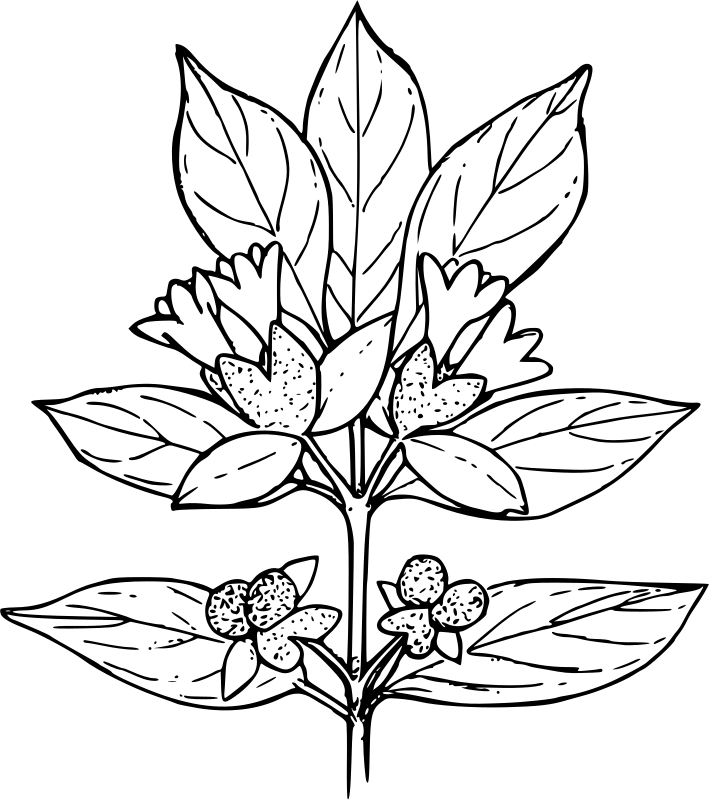
\includegraphics[width=.5\textwidth]{images/flower.png}
  \caption[Kurzfassung der Beschreibung für das Abbildungsverzeichnis]{Lange Version der Beschreibung, die direkt unter der Abbildung gesetzt wird. Es ist wichtig, für jede Abbildung eine umfangreiche Beschreibung anzugeben, da der Leser beim ersten Durchblättern der Arbeit vor allem an den Abbildungen hängen bleibt. Am Besten sollte so die Abbildung mit der dazugehörigen Bildunterschrift ohne weiteren Text verständlich sein und für sich alleine stehen können.}
  \label{fig:flower}
\end{figure}

\begin{figure}
  \centering
  \begin{tikzpicture}[
      node distance=15ex,
      auto,
      on grid,
      shorten >=1pt
    ]
    \node [state, initial] (q0) {$q_0$};
    \node [state, accepting, right=of q0] (q1) {$q_1$};
    \path[->]
      (q0) edge node {$a$} (q1);
  \end{tikzpicture}
  \caption[Graph des Büchi-Automaten $\hat A$.]{Graph des Büchi-Automaten $\hat A$. Der Zustand $q_1$ hat dabei keine ausgehende Kante. Der Zustand ist trotzdem akzeptierend, da beide enthaltenen Zustände von $\acute A$ akzeptierend sind. Die naive Anwendung des Leerheitstests auf alternierenden Büchi-Automaten liefert in diesem Fall also zu viele akzeptierende Zustände.}
  \label{fig:buechi}
\end{figure}

\section{Quelltext}

Quelltext sollte in Abschlussarbeiten nur äußerst sparsam eingesetzt werden. Wichtig ist insbesondere, dass Quelltextauszüge sorgsam ausgewählt und gut erklärt werden.

\begin{lstlisting}[language=Java,gobble=2]
  public class Main {
    // Hello Word in Java
    public static void main(String[] args) {
      System.out.println("Hello World");
    }
  }
\end{lstlisting}

\subsection{Quelltext mit automatischer Nummerierung}

Manchmal möchte man Quelltext eher als Abbildung und nicht als Fließtext behandeln. In diesem Fall soll der Quelltext eine Bildunterschrift und eine automatische Nummerierung erhalten. Die automatische Nummerierung kann dann natürlich auch in Referenzen verwendet werden: In \vref{lst:java} haben wir Java-Quelltext.

\begin{lstlisting}[language=Java,gobble=2,caption={Ich bin die Bildunterschrift des Quelltextes},label=lst:java]
  public class AnotherClass {
    private int number = 0;
    public void add() {
      this.number++;
    }
  }
\end{lstlisting}

Wenn man Quelltext mit Bildunterschrift setzt, muss man darauf achten, dass der Quelltext nach wie vor nicht als Fließumgebung behandelt wird. Entsprechend kann es passieren, dass der Quelltext über zwei Seiten hinweg gesetzt wird. Während das normalerweise nicht stört, kann dieser Umstand in Zusammenhang mit einer Bildunterschrift den Leser irritieren.

\section{Zahlen und Einheiten}

Physikalische Größen sind in Formeln und im Fließtext kursiv zu schreiben, z.B. die Temperatur $T$ und Zeit $t$. Der Index einer physikalischen Größe ist hingegen nicht kursiv zu schreiben, wenn es sich bei diesem Index um eine Variable handelt:

\begin{compactitem}
	\item Index ist Variable: z.B. $T_x$ oder $T_i$
	\item Index ist keine Variable: z.B $T_{\textrm{1}}$ oder $t_{\textrm{off}}$
\end{compactitem}

Es empfiehlt sich, das Paket \textit{siunitx}\footnote{\url{http://ctan.mirror.garr.it/mirrors/CTAN/macros/latex/contrib/siunitx/siunitx.pdf}} für die Darstellung von Zahlen und zugehöriger Einheit zu verwenden. Damit lassen sich Zahlen und kompliziertere Einheiten übersichtlich darstellen, beispielsweise \SI{42}{\kilo\gram\metre\per\square\second}. Weiterhin ist zu beachten:

\begin{compactitem}
	\item einheitenbehaftete Zahlen werden immer mit der dazugehörigen Einheit genannt, geschrieben und nicht voneinander getrennt.
	\item Einheiten werden nicht kursiv geschrieben
	\item Einheiten werden bei der Beschriftung von Graphen oder in Tabellen nicht in eckige Klammern gesetzt, sondern besser wie folgt dargestellt: $c$ in nM oder $c /$mM!
\end{compactitem}

\section{Formeln und Gleichungen}

Formeln und Gleichungen sollten sich nach Möglichkeit in den Lesefluss einfügen und nicht immer nur am Ende des Satzes angehängt werden. Generell sind Gleichungen dabei wie Fließtext zu behandeln, was die Komma- und Punktsetzung betrifft. Außerdem sollten die einzelnen Bestandteile von Formeln und Gleichungen, wie Variablen und Konstanten, immer im Text vor oder nach der entsprechenden Gleichung kurz und knapp erklärt werden. Im Folgenden sind die zuvor genannten Punkte verdeutlicht (entnommen aus \cite{MA_Kappel}):


Unter Verwendung der Bernoullischen Druckgleichung
\begin{equation}
	\label{eq:bernoulli_pressure}
	p_{\text{s}} +  \varrho_{\text{s}} g z_{\text{s}} + \frac{1}{2} \varrho_{\text{s}} v^{2}_{\text{s}} = p_{\text{a}} + \varrho_{\text{a}} g z_{\text{a}} + \frac{1}{2} \varrho_{\text{a}} v^{2}_{\text{a}}
\end{equation}
kann ein alternativer Ausdruck für $ p_{s} $ gefunden werden. Hier stehen $ p_{\text{s}} $ und $ p_{\text{a}} $ für den Druck innerhalb der Spritze bzw. am Ausgang der Spritze, $ \varrho $ beschreibt die Dichte des Fluids, und $ v_{\text{s}} $ und $ v_{\text{a}} $ für die Geschwindigkeit des Fluids innerhalb der Spritze bzw. am Ausgang. 
Die Lage, oder auch die geodätische Höhe, der Spritze und des Ausgangs wird hier mit $ z_{\text{a}} $ bzw. $ z_{\text{s}} $ beschrieben, und $ g $ steht für die Fallbeschleunigung im Schwerefeld der Erde.
Aufgrund der Annahme, dass das verwendete Fluid inkompressibel ist, also $ \varrho_{\text{s}} = \varrho_{\text{a}} = \varrho = const. $ gilt, kann Gleichung \ref{eq:bernoulli_pressure} auch wie folgt geschrieben werden:
\begin{equation}
	\label{eq:bernoulli_pressure_rearranged}
p_{\text{s}} +  \varrho g z_{\text{s}} + \frac{1}{2} \varrho v^{2}_{\text{s}} = p_{\text{a}} + \varrho g z_{\text{a}} + \frac{1}{2} \varrho v^{2}_{\text{a}} \, .
\end{equation}

\section{Hinweise zu Form und Stil}

Es ist auf einen präzisen Schreibstil zu achten. Umschreiben Sie keine Sachverhalte, die Sie auch konkret benennen können. Beachten Sie beim Verfassen Ihrer Arbeit außerdem diese weiteren Punkte:

\begin{compactitem}
	\item Drücken Sie sich möglichst im Passiv aus (nicht \frqq\textit{man} tut dies und jenes\flqq{}).
	\item Vermeiden Sie Sätze im Imperativ, Umgangssprache und unnötige Füllwörter.
	\item Es sollten \textit{Laborslang }und englische Begriffe vermieden werden, z.B. \frqq Aufbau\flqq{} statt \frqq Setup\flqq{} und \frqq ROXS\flqq{}  statt \frqq Zaubercocktail\flqq.
	\item Erklären Sie Abkürzungen bei ihrer ersten Verwendung, und nehmen Sie diese in das Abkürzungsverzeichnis auf.
	\item Lateinische Begriffe sollten immer kursiv dargestellt werden, wie z.B. \textit{in vivo}.
\end{compactitem}
  \include{ergebnisse}
  %!TEX root = thesis.tex

\chapter{Diskussion}
\label{chapter:diskussion}

Der folgende Abschnitt ist einem Leitfaden der Universität Bremen \cite{uni-bremen} entnommen:
Häufig fällt es bei der ersten wissenschaftlichen Arbeit schwer, seine Untersuchungsergebnisse zu erörtern bzw. seine Diskussion zu strukturieren. Oft ist es sinnvoll, in der Reihenfolge zu diskutieren, wie die Ergebnisse (Versuche) im Ergebnisteil dargestellt sind. Dies ist aber kein Muss. Ziel sollte jedoch eine Synthese der eigenen Ergebnisse sein. Es lässt sich dabei kaum vermeiden, Teile der Ergebnisse noch einmal aufzugreifen, um daran anzuknüpfen. Jedoch sind reine Ergebnisaufzählungen zu vermeiden. Prinzipiell sollte eine Diskussion folgende Fragen beantworten:

\begin{compactitem}
  \item In welchem Verhältnis stehen meine Ergebnisse zu den bereits bekannten Daten?
  \item Wie lautet die Antwort auf die eingangs formulierten Fragen/ Hypothesen?
  \item Welche Relevanz haben meine Ergebnisse?
\end{compactitem}

Zur Beantwortung dieser Fragen ist es essentiell, sich mit Studien und Ergebnissen anderer Autoren kritisch auseinander zu setzen, diese zu den eigenen Erkenntnissen in Beziehung zu setzen und zu kommentieren. Genau dieser Prozess beschreibt, was wissenschaftliches Schreiben ausmacht. Das Zitieren von relevanter Literatur ist somit unumgänglich. Bereits in der Einleitung haben Sie einen Überblick zu ihrer Thematik gegeben. Jetzt ist es wichtig, einen Vergleich mit ähnlichen Untersuchungen, im Hinblick auf die in der Einleitung aufgeworfenen Fragen und Hypothesen, zu geben. In diesem Kontext wird auch eine kritische Betrachtung der eigenen Methodik etc. erwartet (Fehlerdiskussion). Spekulationen, d.h. Mutmaßungen oder Annahmen über Sachverhalte, sind generell zu vermeiden. Wenn diese aber hilfreich für das Verständnis oder die Gedankenführung sind, müssen diese Meinungen oder Vermutungen als solche erkennbar werden.
Die Diskussion sollte am Ende eine Schlussfolgerung, am besten einen Erkenntnisgewinn, ermöglichen. Diese gibt nicht wieder, was gerade in der Diskussion bewertet wurde, sondern sollte die Diskussion zusammenfassen (was hat diese Untersuchung gebracht und welche Fragen wurden beantwortet) und einen Ausblick auf weiterführende Untersuchungen geben.


  \include{fazit}

  \appendix

  %!TEX root = thesis.tex

\chapter{Anhang}

Dieser Anhang enthält tiefergehende Informationen, die nicht zur eigentlichen Arbeit gehören.

\section{Abschnitt des Anhangs}

In den meisten Fällen wird kein Anhang benötigt, da sich selten Informationen ansammeln, die nicht zum eigentlichen Inhalt der Arbeit gehören. Vollständige Quelltextlistings haben in ausgedruckter Form keinen Wert und gehören daher weder in die Arbeit noch in den Anhang. Darüber hinaus gehören Abbildungen bzw. Diagramme, auf die im Text der Arbeit verwiesen wird, auf keinen Fall in den Anhang.


  \backmatter

  \cleardoublepage
  \phantomsection
  \pdfbookmark{Abbildungsverzeichnis}{listoffigures}
  \listoffigures

  \cleardoublepage
  \phantomsection
  \pdfbookmark{Tabellenverzeichnis}{listoftables}
  \listoftables

%  \cleardoublepage
%  \phantomsection
%  \pdfbookmark{Definitions- und Theoremverzeichnis}{listoftheorems}
%  \renewcommand{\listtheoremname}{Definitions- und Theoremverzeichnis}
%  \listoftheorems[ignoreall,show={Lemma,Theorem,Korollar,Definition}]

  \cleardoublepage
  \phantomsection
  \pdfbookmark{Quelltextverzeichnis}{listoflistings}
  \lstlistoflistings

  \include{abkuerzungen}

  \cleardoublepage
  \phantomsection
  \pdfbookmark{Literaturverzeichnis}{bibliography}
  \bibliography{literature}
\end{document}
